%%%%%%%%%%%%%%%%%%%%%%%%%%%%%%%%%%%%%%%%
% datoteka diploma-vzorec.tex
%
% vzorčna datoteka za pisanje diplomskega dela v formatu LaTeX
% na UL Fakulteti za računalništvo in informatiko
%
% vkup spravil Gašper Fijavž, december 2010
% množica popravkov v januarju, februarju marcu 2011
% verzija 29. marec 2011

\documentclass[a4paper, 12pt]{book}

\usepackage{color}
\usepackage{xcolor}
\usepackage{listings}
\usepackage{caption}
\DeclareCaptionFont{white}{\color{white}}
\DeclareCaptionFormat{listing}{\colorbox{gray}{\parbox{\textwidth}{#1#2#3}}}
\captionsetup[lstlisting]{format=listing,labelfont=white,textfont=white}

\usepackage[utf8x]{inputenc}   % omogoča uporabo slovenskih črk kodiranih v formatu UTF-8 
\usepackage[slovene,english]{babel}    % naloži, med drugim, slovenske delilne vzorce
\usepackage[pdftex]{graphicx}  % omogočam vlaganje slik različnih formatov 
\usepackage{fancyhdr}          % poskrbi, na primer, za glave strani
\usepackage{amssymb}           % dodatni simboli
\usepackage{amsmath}           % eqref, npr.
\usepackage{subfig}

\graphicspath{{./images/}, {./dia/}}


\renewcommand{\baselinestretch}{1.3} % ustrezen razmik med vrsticami

%oznake strani
\renewcommand{\chaptermark}[1]%
{\markboth{\MakeUppercase{\thechapter.\ #1}}{}} \renewcommand{\sectionmark}[1]%
{\markright{\MakeUppercase{\thesection.\ #1}}} \renewcommand{\headrulewidth}{0.5pt} \renewcommand{\footrulewidth}{0pt} 
\fancyhf{}
\fancyhead[LE,RO]{\sl \thepage} \fancyhead[LO]{\sl \rightmark} \fancyhead[RE]{\sl \leftmark}

\newcommand{\BibTeX}{{\sc Bib}\TeX}

\newcommand{\autfont}{\Large}
\newcommand{\titfont}{\LARGE\bf}
\newcommand{\clearemptydoublepage}{\newpage{\pagestyle{empty}\cleardoublepage}}
\setcounter{tocdepth}{1}	      % globina kazala

% konstrukti
\newtheorem{izrek}{Izrek}[chapter]
%\newtheorem{trditev}{Trditev}[izrek]
\newenvironment{dokaz}{\emph{Dokaz.}\ }{\hspace{\fill}{$\Box$}}

\begin{document}
\selectlanguage{slovene}
\frontmatter
\setcounter{page}{1} %
\renewcommand{\thepage}{}       % preprecimo težave s številkami strani v kazalu 

%%%%%%%%%%%%%%%%%%%%%%%%%%%%%%%%%%%%%%%%
%naslovnica
 \thispagestyle{empty}%
   \begin{center}
    {\large\sc Univerza v Ljubljani\\%
      Fakulteta za računalništvo in informatiko}%
    \vskip 10em%
    {\autfont Gregor Majcen\par}%
    {\titfont Oddaljeno vodenje mobilne platforme s pametnim telefonom \par}%
    {\vskip 2em \textsc{DIPLOMSKO DELO\\[2mm] 
    VISOKOŠOLSKI STROKOVNI ŠTUDIJSKI PROGRAM PRVE STOPNJE RAČUNALNIŠTVO IN INFORMATIKA}\par}%
    \vfill\null%
    {\large \textsc{Mentor}: doc.\ dr.  Danijel Skočaj\par}%
    {\vskip 2em \large Ljubljana 2011 \par}%
\end{center}
% prazna stran
\clearemptydoublepage

%%%%%%%%%%%%%%%%%%%%%%%%%%%%%%%%%%%%%%%%
%copyright stran
\thispagestyle{empty}
\vspace*{8cm}
{\small \noindent
Rezultati diplomskega dela so intelektualna lastnina Fakultete za ra\-ču\-nal\-niš\-tvo in informatiko Univerze v Ljubljani. 
Za objavljanje ali izkoriščanje rezultatov di\-plom\-ske\-ga dela je potrebno pisno soglasje Fakultete za ra\-ču\-nal\-niš\-tvo in 
informatiko ter mentorja.}


% prazna stran
\clearemptydoublepage

%%%%%%%%%%%%%%%%%%%%%%%%%%%%%%%%%%%%%%%%
% stran 3 med uvodnimi listi
%\noindent
%Namesto te strani {\bf vstavite} original izdane teme diplomskega 
%dela s podpisom mentorja in dekana ter žigom fakultete, ki ga diplomant
%dvigne v študent\-skem referatu,  preden odda izdelek v vezavo!
%Glej tudi sam konec Poglavja~\ref{ch2} na strani~\pageref{pp}.

\clearemptydoublepage

% prazna stran
\clearemptydoublepage

%%%%%%%%%%%%%%%%%%%%%%%%%%%%%%%%%%%%%%%%
% izjava o avtorstvu
\vspace*{1cm}
\begin{center} 
{\Large \textbf{\sc Izjava o avtorstvu diplomskega dela}}
\end{center}

\vspace{1cm}
\noindent Spodaj podpisani Gregor Majcen,
z vpisno številko \textbf{63070199}, sem avtor  diplomskega dela z naslovom:
   
\vspace{0.5cm}
\emph{Oddaljeno vodenje mobilne platforme s pametnim telefonom}

\vspace{1.5cm}
\noindent S svojim podpisom zagotavljam, da:
\begin{itemize}
	\item sem diplomsko delo izdelal samostojno pod mentorstvom 
		doc.\ dr.\ Danijela Skočaja,

	\item	so elektronska oblika diplomskega dela, naslov (slov., angl.), povzetek (slov., angl.) ter ključne besede (slov., angl.) identični s tiskano obliko diplomskega dela
	\item soglašam z javno objavo elektronske oblike diplomskega dela v zbirki ``Dela FRI''.
\end{itemize}

\vspace{1cm}
\noindent V Ljubljani, dne 15. septembra 2011 \hfill Podpis avtorja:

% prazna stran
\clearemptydoublepage

%%%%%%%%%%%%%%%%%%%%%%%%%%%%%%%%%%%%%%%%
% zahvala
\thispagestyle{empty}\mbox{}\vfill\null\it%
Zahvaljujem se mentorju doc. dr. Danijelu Skočaju za vso strokovno pomoč in material za izdelavo diplomskega dela. 

Poleg mentorja se zahvaljujem tudi as. mag. Luku Čehovinu za sprotno pomoč pri izdelavi vsakega dela v laboratorju in preko e-pošte. 

Zahvaljujem se sošolcu Mihu Zidarju za pomoč pri delu s strojno opremo, spajkanju in testiranju.

Da pa nismo obupali nad spodaj opisanim usmerjevalnikom se zahvaljujem Zoranu Krsniku, dipl. inž. el. za uspešno odkrite napake in narejen RS232 konverter.

Zahvaljujem se vsem, ki so mi kakorkoli pomagali pri diplomskem delu in staršem za omogočen študij.
\rm\normalfont

% prazna stran
\clearemptydoublepage

%%%%%%%%%%%%%%%%%%%%%%%%%%%%%%%%%%%%%%%%%
%% posvetilo
%\thispagestyle{empty}\mbox{}{\vskip0.20\textheight}\mbox{}\hfill\begin{minipage}{0.55\textwidth}%
%Svoji dragi Alenčici.
%\normalfont\end{minipage}
% 
%% prazna stran
%\clearemptydoublepage

%%%%%%%%%%%%%%%%%%%%%%%%%%%%%%%%%%%%%%%%
% kazalo
\def\thepage{}% preprecimo tezave s stevilkami strani v kazalu 
\tableofcontents{}


% prazna stran
\clearemptydoublepage

%%%%%%%%%%%%%%%%%%%%%%%%%%%%%%%%%%%%%%%%
% povzetek 
\addcontentsline{toc}{chapter}{Povzetek}
\chapter*{Povzetek}
Diplomsko delo govori o mobilni platformi, ki jo upravljamo s pametnim telefonom. Za mobilno platformo je uporabljen sesalec iRobot Roomba, na katerem sta pritrjena usmerjevalnik in kamera. Vzpostavitev povezave med pametnim telefonom in mobilno platformo dosežemo preko interneta. Pametni telefon je uporabljen kot igralna konzola, s katero upravljamo gibanje mobilne platforme. 
% prazna stran
\clearemptydoublepage

%%%%%%%%%%%%%%%%%%%%%%%%%%%%%%%%%%%%%%%%
% abstract
\selectlanguage{english}
\addcontentsline{toc}{chapter}{Abstract}
\chapter*{Abstract}
This thesis describes a system for remote control of a mobile platform using a smartphone. As a mobile platform is used an iRobot Roomba vacuum cleaner equipped with a wireless router and a camera. The mobile platform and the smartphone communicate over the internet. The smartphone is used as a gaming console to control the movement of the mobile platform. 
\selectlanguage{slovene}
% prazna stran
\clearemptydoublepage

%%%%%%%%%%%%%%%%%%%%%%%%%%%%%%%%%%%%%%%%
\mainmatter
\setcounter{page}{1}
\pagestyle{fancy}

\chapter{Uvod}
Brez tehnologije je danes skoraj nemogoče živeti. Spremlja nas na vsakem koraku, pa naj bo to telefon, avtomobil, televizija, računalnik,... Vzemimo na primer osebni računalnik. Prve naprave, ki so približno podobne današnjim osebnim računalnikom so se pojavile približno 70 let nazaj. Od takrat pa vse do danes in še vedno razvoj poteka izjemno hitro. Ra\-ču\-nal\-ni\-ki postajajo vse manjši, bolj zmogljivi in bolj varčni z energijo. Strukturo so prenesli tudi na telefone, ki jih imenujemo pametni telefoni. Pametni telefoni so na voljo šele kako desetletje, prodaja le teh pa iz dneva v dan narašča. Na začetku izida pametnih telefonov je veliko ljudi, vključno z mano, govorilo, da takega telefona ne potrebujejo, enostavno ker je telefon namenjen telefoniranju. Enako so še pred tem ljudje govorili za osebni računalnik in televizijo. {\it ``V času ko je izšla prva televizija so vsi govorili, da je ne potrebujejo. Čez nekaj let so jo imeli skoraj vsi. Enako se je zgodilo z osebnim računalnikom, danes skoraj ni družine, kjer ne bi bila vsaj ena televizija in en osebni računalnik. Danes se razvijajo roboti, ki opravljajo dela namesto nas. Še pred nekaj leti so vsi govorili, da je to le za osebe s preveč denarja in da ni za vsakdanje gospodinjstvo. Danes se vse več ljudi odloča za na primer avtomatski sesalec in iz vsega skupaj lahko sklepamo, da čez nekaj let ne bo niti enega gospodinjstva brez kakega robota.''} je nekoč povedal mentor na predavanju.

Tehnologija torej vstopa v naše življenje, nam omogoča nove aplikacije. Različne tehnologije služijo različnim opravilom, kar pa še ne pomeni, da je kombinacija le teh nemogoča. Predstavljajmo si, da smo v službi in želimo malo pogledati, kaj se dogaja v stanovanju. Za kaj takega je potrebna kamera, ki nam omogoča video sliko. Najboljša rešitev za dostop do kamere je internet, saj imamo s pomočjo interneta oddaljeno video sliko. Potreben je tudi prikaz slike, ampak za to potrebujemo napravo, ki nam to omogoča. Najlažja možnost je s telefonom, ki je običajno vedno pri roki. Preko telefona vzpostavimo povezavo z internetom in kamero ter tako opazujemo trenutno dogajanje v stanovanju. Kaj pa, če želimo pogledati tudi v spalnici, kjer kamere ni, ta pa tudi nima koles, da bi se lahko premikala. Ker kamera ni zelo velika naprava jo lahko postavimo kamorkoli, tudi na mobilno platformo, ki pa ima kolesa in s tem dosežemo da imamo ``kamero na kolesih''. Prej je omenjeno, da za sliko iz kamere uporabimo telefon in ta isti telefon uporabimo tudi za premikanje mobilne platforme. Sedaj nam nič več ne more uiti. 

Primer nadzora stanovanja je dober primer za uporabnost našega di\-plom\-ske\-ga dela. V naslednjih poglavjih je opisan celotni sistem delovanja sistema in vse naprave, ki so potrebne za delovanje. Najprej je opisana {\tt zasnova sistema}, kjer je na kratko povzet cilj in zahteva celotnega sistema. V naslednjih poglavjih so podatki o vsaki napravi posebej. V poglavju o {\tt mobilni platformi} je opisana uporaba za premikanje po ravni površini. Nastavitve za brezžično komunikacijo med mobilno platformo in zunanjo napravo so opisana v poglavju {\tt brezžični prenos podatkov}, kjer je predstavljena naprava in vse njene nadgradnje. Kot zadnja naprava je opisan {\tt pametni telefon} in razvoj programa, ki je potreben za nadzor mobilne platforme. Predzadnje poglavje je podobno kot začetno, le da tokrat poznamo že vse naprave, potrebne za delovanje, in zato opišemo celotno {\tt delovanje sistema} bolj podrobno. Na koncu so podane še {\tt sklepne ugotovitve}, kjer je opisano delovanje posamezne naprave v vsakdanjem življenju. 

\chapter{Zasnova sistema}

Cilj celotnega sistema je upravljati mobilno platformo ne glede na našo trenutno lokacijo, kot je prikazano na sliki~\ref{diaCilj}. To je mogoče zagotoviti le s pomočjo internetne povezave, zato potrebujemo na lokaciji mobilne platforme in trenutni lokaciji uporabnika napravi, ki omogočata internetno povezavo. Današnji telefoni že omogočajo internetno povezavo, zato so primerni za upravljalnike mobilne platforme.

\begin{figure}[h]
	\centering
	\includegraphics[width=0.75\textwidth]{cilj}
	\caption{Cilj sistema}
	\label{diaCilj}
\end{figure}

Tudi mobilna platforma mora imeti možnost povezave do interneta in slike vožnje, zato jo moramo še nadgraditi. Na osnovni model mobilne platforme dodamo usmerjevalnik, ki nam služi kot vmesnik med mobilno platformo, kamero in internetno povezavo, kot je prikazano na sliki~\ref{diaShema}. Da ohranimo mobilnost uporabimo brezžično omrežje.

\begin{figure}[h]
	\centering
	\includegraphics[width=0.75\textwidth]{shema}
	\caption{Groba zasnova sistema}
	\label{diaShema}
\end{figure}

Celoten sistem je torej sestavljen iz več naprav, ki jih podrobneje opišemo v naslednjih poglavjih.

\chapter{Mobilna platforma}
Beseda platforma ima v svetu veliko pomenov, v našem primeru pa jo uporabljamo kot ime za manjšega robota, ki ima možnost premikanja po prostoru. Lastnost premikanja po prostoru imenujemo tudi mobilnost. Zaradi teh dveh lastnosti je naš robot poimenovan {\tt mobilna platforma}.

\begin{figure}[h]
	\centering
	\subfloat{\label{picRobot_no1}\includegraphics[height=3.7cm]{robot_no1}} \hfill
	\subfloat{\label{picRobot_no2}\includegraphics[height=3.7cm]{robot_no2}} \hfill
	\subfloat{\label{picRobot_no3}\includegraphics[height=3.7cm]{robot_no3}} \hfill
	\caption{Različne implementacije mobilne platforme}
	\label{picRobot}
\end{figure}

Zaradi cenovne ugodnosti, dostopnosti, nosilnosti, robustnosti in razloga, da mobilna platforma ne bi bila uporabna le za ta projekt smo se odločili za uporabo naprave iRobot Roomba. 

\section{iRobot Roomba}
iRobot Roomba je avtomatski sesalec, ki je vse bolj priljubljen in pri nekaterih nujen pripomoček v gospodinjstvu, kar potrjuje tudi podatek, da je bilo v šestih letih obstoja prodano kar 2.5 milijona naprav. Sesalec Roomba je bil predstavljen leta 2002, še istega leta pa je prva generacija tudi prišla v prodajo. Do danes obstajajo tri različne generacije. Lastnosti avtomatskega sesalca se po generaciji ne razlikujejo veliko, vsaka generacija ima svoje nadgradnje, to je število senzorjev za bolj učinkovito vožnjo in različno obliko sesalca. Poleg teh dveh pa je najpomembnejša razlika med prvo in drugo generacijo sposobnost, da se sesalec sam napolni, ko se izprazni~\cite{bibWikiRoomba}. 

\begin{figure}[h]
	\centering
	\subfloat[prva generacija]{\label{picRoomba_no1}\includegraphics[height=3.7cm]{roomba_no1}} \hfill
	\subfloat[druga generacija]{\label{picRoomba_no2}\includegraphics[height=3.7cm]{roomba_no2}} \hfill
	\subfloat[tretja generacija]{\label{picRoomba_no3}\includegraphics[height=3.7cm]{roomba_no3}} \hfill
	\caption{Vse tri generacije iRobot Roomba}
	\label{picRobot}
\end{figure}

\section{Komunikacijski vmesnik}
Že od samega začetka sesalci Roomba vsebujejo tudi vmesnik za nadzor platforme. ROI (Roomba Open Interface), kot so ga poimenovali je 7-nožični {\tt Mini-DIN} konektor, ki podpira TLL zaporedni vmesnik. Ker želimo sesalec Roomba upravljati preko zunanje naprave, je ta konektor izjemnega pomena, da pa se konektor lahko uporablja, je potrebno zgraditi pretvornik, ki ROI pretvori v standardni 9-nožični zaporedni konektor (RS232).

Kot je prikazano na sliki~\ref{picROIshema}, za pretvornik potrebujemo čip MAX232, ki je namenjen dvigu napetosti signala na 12V. Potrebna sta tudi oba konektorja, Mini-DIN in RS232. Namesto Mini-DIN konektorja lahko uporabimo tudi 8-nožični Mac zaporedni konektor (ang. Mac serial port), ki je lažje dobavljiv. V tem primeru je potrebno paziti na številčenje nožic v konektorju, kot je prikazano na levi strani slike~\ref{picROIshema}. 

Pretvornik je mogoče narediti na nekaj kvadratnih centimetrov velike ploščice, na kateri je izdelana celotna shema, kar je razvidno na sliki~\ref{picROI}.

\begin{figure}[h]
	\centering
	\includegraphics[width=0.75\textwidth]{ROI}
	\caption{Shema pretvornika iz ROI v RS232~\cite{bibRoombaROI}}
	\label{picROIshema}
\end{figure}

\begin{figure}[h]
	\centering
	\includegraphics[width=0.5\textwidth]{ROIfull}
	\caption{Pretvornik iz ROI v RS232~\cite{bibRoombaROI}}
	\label{picROI}
\end{figure}

Različne generacije sesalca Roomba uporabljajo različne hitrosti prenosa ROI vmesnika. Za naš projekt smo si izbrali najnovejšo, to je tretja generacija Roombe, serije 5xx. ROI vmesnik pri tej seriji uporablja hitrost 115200 b/sec. Preden pa začnemo z zunanjim vodenjem moramo poznati cikel stanj, ki ga sesalec Roomba uporablja. 

Ko je sesalec Roomba ugasnjen, je v stanju spanja (ang. {\tt sleep}). S pritiskom na vrhnji gumb POWER se sesalec Roomba prižge (ang. {\tt on}) in je pripravljen za sprejemanje ukazov preko ROI vmesnika. Na začetku je potrebno sesalec Roomba inicializirati, kar storimo z ukazoma START in CONTROL. Z ukazom START sesalec Roomba postavimo v pasivno stanje (ang. {\tt passive}), z ukazom CONTROL pa v varno stanje (ang. {\tt safe}). V varnem stanju imamo popoln nadzor nad sesalcem Roomba in lahko uporabljamo vse njegove lastnosti. V primeru, da z zunanjim dostopom sesalec Roomba izgubi stik s tlemi, se zaradi varnega stanja vrne v pasivno stanje. To varnostno lastnost lahko izklopimo z ukazom FULL, ki sesalec Roomba postavi v polno stanje (ang. {\tt full}). S ponovnim pritiskom na gumb POWER ali z ukazom POWER se sesalec Roomba vrne v stanje spanja, dokler ponovno ne pritisnemo gumba. Cikel je bolje razviden na sliki~\ref{picRoombaStatus}. 


\begin{figure}[h]
	\centering
	\includegraphics[width=0.75\textwidth]{roomba_status}
	\caption{Statusni cikel Roombe~\cite{bibHackRoomba}}
	\label{picRoombaStatus}
\end{figure}

Ko smo v varnem stanju, lahko začnemo z zunanjem vodenjem. Za vožnjo uporabimo ukaz DRIVE, ki za parametra potrebuje hitrost in radij, podana v milimetrih. Najvišja hitrost za sesalec Roomba je 500mm/s, če pa podamo negativno hitrost to pomeni vzvratna vožnja. Radij ima razpon od -2000mm do 0, kar povzroči zavijanje levo in od 0 do 2000mm desno. Kot zavoja je odvisen od hitrosti. Izjema je radij 32768 oziroma hexadecimalno 0x8000 kar pomeni naravnost naprej. Radij nam določa hitrost za vsako kolo posebej, nastavljeno z enačbo $V_{levo} = V(1-\frac{129}{r})$ in $V_{desno} = V(1+\frac{129}{r})$, kjer je r radij in V hitrost. 

Da je upravljanje s sesalcem Roomba lažje, je uporabljen že izdelan programski vmesnik {\tt roombacmd}\footnote{Program je dostopen na {\tt http://roombahacking.com/software/roombacmd/}~\cite{bibRoombacmd}}.

\section{Programski vmesnik}
Roombacmd je program napisan v programskem jeziku C. Je terminalski (ang. console) program, ki sprejme parametre ob zagonu in se po končanem delu zapre. Ob zagonu programa roombacmd brez parametrov se nam prikaže pomoč za uporabo parametrov, kot je prikazano na sliki~\ref{picRoombacmd}. 

\begin{figure}[h]
	\centering
	\includegraphics[width=0.9\textwidth]{roombacmd}
	\caption{Pomoč programa roombacmd}
	\label{picRoombacmd}
\end{figure}

Izvorna koda programa roombacmd je sestavljena iz dveh datotek. Prva datoteka, {\tt roombacmd.c}, je le razčlenjevalnik vnesenih parametrov (ang. par\-ser). Glavno funkcionalnost za upravljanje sesalca Roomba pa vsebuje datoteka {\tt roombalib.c}, kjer so napisani vsi ukazi. Ker je bil program roombacmd napisan v času druge generacije sesalcev Roomba, je program potrebno malo priredili. Druga generacija je delovala s hitrostjo pošiljanja podatkov 57600b/sec, kar je pri tretji generaciji spremenjeno na 115200b/sec. Ker program roombacmd podpira le vožnjo naprej, nazaj in okrog svoje osi, je potrebno dodati tudi funkcijo zavojev. Dodan je nov parameter ``R'', s katerim določimo radij v razponu od -2000 do 2000. Ker program roombacmd z vsakim zagonom zažene ukaza START in CONTROL, s tem povzroči nekaj milisekundi zamik, je to odpravljeno z novim parametrom ``i'', ki ne potrebuje nobenega atributa. Ukaza START in CONTROL se torej kličeta le ob nastavitvi parametra ``i''.

\section{Kamera}
Programski vmesnik je namenjen le vožnji, naša mobilna platforma pa potrebuje še vidno sliko vožnje. Na sesalec Roomba je zato pritrjena kamera AXIS 215 PTZ, ki je tudi prikazana na sliki~\ref{picKamera}. To je mrežna oziroma IP kamera, ki se jo upravlja preko spletnega vmesnika. 

\begin{figure}[h]
	\centering
	\includegraphics[width=0.3\textwidth]{kamera}
	\caption{Kamera AXIS 215 PTZ~\cite{bibKamera}}
	\label{picKamera}
\end{figure}

Kamera je zelo prilagodljiva, saj omogoča pogled v vse smeri. Tak tip kamere je v vsakdanjem življenju primeren kot varnostna kamera, saj poleg pogleda v vse smeri omogoča tudi dnevno/nočno funkcionalnost (ang. Day/Night function) s pomočjo IR senzorja. Zelo učinkovita je tudi pri približevanju predmetov, saj ima možnost 48-kratnega povečanja slike. Podatke prenaša preko mrežnega kabla, trenutna slika pa je dostopna preko spletnega programskega vmesnika (ang. application program interface - API).

\chapter{Brezžični prenos podatkov}
Brezžični prenos podatkov je zagotovljen preko usmerjevalnika (ang. router). Dandanes je na trgu veliko usmerjevalnikov, ki imajo bolj ali manj podobno funkcionalnost. Večinoma se razlikujejo po zmogljivosti strojne opreme in opremljenosti grafičnega vmesnika, ki ga lahko odpremo s spletnim brskal\-nikom (ang. browser). 

Za naš projekt smo izbrali Linksys WRT54GL, ki je prikazan na sliki~\ref{picLinksysWRT54GL}. Linksys WRT54GL je zaradi cenovne ugodnosti in kar dobre zmogljivosti eden izmed najbolj priljubljenih usmerjevalnikov za navadne uporabnike. O\-prem\-ljen je z arhitekturo MIPS proizvajalca Broadcom. Čeprav procesor (ang. central processing unit - CPU) teče pri 200MHz in ima le 16MB pomnilnika (ang. random access memory - RAM), je dovolj zmogljiv in varčen za naš problem. Poleg prej naštetega ima tudi najpomembnejša elementa našega projekta: možnost brezžičnega omrežja (ang. wireless) in nožice (ang. pins) za zaporedna vrata (ang. serial port). Namesto zaporednih vrat bi lahko uporabili USB (ang. universal serial bus), ki je bolj enostaven in dandanes veliko pogosteje uporabljen kot zaporedna vrata. Ker takšnega usmerjevalnika ni bilo na voljo, smo se vseeno odločili za Linksys WRT54GL.

\begin{figure}[h]
	\centering
	\includegraphics[width=0.75\textwidth]{LinksysWRT54GL}
	\caption{Linksys WRT54GL}
	\label{picLinksysWRT54GL}
\end{figure}

\section{Brezžično omrežje}
Kot skoraj vsak novejši usmerjevalnik ima tudi WRT54GL vgrajen čip za upravljanje z brezžičnim omrežjem in sicer Broadcom BCM43xx 802.11b/g. Omogoča nam brezžično povezavo do usmerjevalnika in nazaj. Bistvo brez\-žičnega omrežja je, da nismo omejeni na dolžino kabla, temveč na moč brezžičnega signala. Ker si želimo našo mobilno platformo, v našem primeru sesalec Roomba, narediti brezžično, je to obvezno. Možna sta dva principa brezžične povezave.

Prva možnost je, da se nastavi omrežna točka (ang. access point) in se lahko poveže le v bližini usmerjevalnika. Ta možnost je zelo enostavna in ne potrebuje veliko nastavitev (potrebno je nastaviti le ime omrežja in stopnjo varnosti), vendar smo omejeni na zmogljivost anten usmerjevalnika, za naš sistem pa je potrebno oddaljeno vodenje. To je možno le, če se povežemo na globalno omrežje (ang. wide area network - WAN).

To je druga možnost, in sicer da se usmerjevalnik nastavi kot odjemalec (ang. client). Za to potrebujemo še eno omrežno točko, ki je preko mrežnega kabla povezana na globalno omrežje. Tu pa se stvari že zapletejo, saj originalni uporabniški vmesnik za nastavitev povezave tega ne omogoča. Na voljo je kar nekaj neuradnih različic operacijskega sistema (ang. firmware) kot na primer DD-Wrt, Tomato, FreeWRT, X-WRT, OpenWRT,... Odločili smo se za OpenWRT, ki je opisan v poglavju~\ref{sec:OpenWRT}. 

\section{Zaporedni vhod}
Zaporedna vrata so alternativa USB-ju, ki nam jo omogoča naš usmerjevalnik. Omogočajo nam komuniciranje usmerjevalnika z zunanjo vhodno-izhodno napravo (ang. input/output device - I/O device). Vezava zaporednih vrat na usmerjevalnik izniči garancijo, saj pomeni poseg v notranjost usmerjevalnika in ročno integracijo. Na ploščici (ang. board) so le nožice, saj se ponavadi uporabljajo samo za reševanje programsko pokvarjenih usmerjevalnikov (ang. bricked router) in niso namenjene navadnim uporabnikom. Reža (ang. slot), kjer se nahajajo nožice, je postavljena desno zgoraj, označena z JP2, kot je prikazano na sliki~\ref{picJP2}. Vsega skupaj je nameščenih deset nožic, za vsaka zaporedna vrata pa potrebujemo štiri, kar pomeni da imamo na voljo dvoje zaporednih vrat, ki so poimenovana kot ttyS0 in ttyS1, dve nožici pa sta brez povezave. Pomen nožic je podrobneje opisan v tabeli~\ref{tabJP2}. 

\begin{figure}[h]
	\centering
	\includegraphics[width=0.75\textwidth]{JP2}
	\caption{JP2 reža~\cite{bibJbproject}}
	\label{picJP2}
\end{figure}

\begin{table}[h]
	\centering
	\begin{tabular}{|l|l|l}
		\cline{1-2}
		Pin 1: 3.3V & Pin 2: 3.3V  \\ \cline{1-2}
		Pin 3: Tx (ttyS1) & Pin 4: Tx (ttyS0) \\ \cline{1-2}
		Pin 5: Rx (ttyS1) & Pin 6: Rx (ttyS0) \\ \cline{1-2}
		Pin 7: NC & Pin 8: NC \\ \cline{1-2}
		Pin 9: GND & Pin 10: GND \\ \cline{1-2}
	\end{tabular}
	\caption{Nožice na JP2 reži~\cite{bibJbproject}}
	\label{tabJP2}
\end{table}

Zaporedna vrata na usmerjevalniku komunicirajo s TTL signali pri na\-pe\-to\-sti 3.3V. Ker komuniciramo le z eno zunanjo napravo, potrebujemo le ena zaporedna vrata. Odločili smo se za ttyS1, ker na ttyS0 sistem pošilja vsa sporočila (ang. debug, warrning messages) jedra (ang. kernel), kar je sicer pri reševanju usmerjevalnika v zelo veliko pomoč, vendar je za nas moteče. 

Da vse skupaj standardiziramo v RS232, moramo napetost signala dvigniti na 12V. Za to potrebujemo pretvornik (ang. converter).

\subsection{Izdelava in integracija pretvornika}
Izdelati moramo pretvornik, ki napetost signala zaporednih vrat usmerjevalnika dvigne iz 3.3V na 12V. Tako dosežemo standard RS232 in s tem možnost komuniciranja z večino naprav. Najboljši in najlažji način je uporaba čipa MAX232, ki je na voljo v večini elektronskih trgovin. En čip zadostuje za dvoje zaporednih vrat, vendar mi potrebujemo le ena. Kot izhod iz čipa uporabimo 9-nožični RS232 konektor. Obstajata dva različna tipa RS232 konektorja: moški(ang. male connector) in ženski (ang. female connector). Večina osebnih računalnikov (ang. personal computer - PC) ima moški konektor. Naša mobilna platforma ima ženski konektor in zato za povezavo potrebujemo moški konektor, kot ga ima osebni računalnik. 

\begin{figure}[h]
	\centering
	\includegraphics[width=0.75\textwidth]{max232}
	\caption{shema uporabe MAX232~\cite{bibJbproject}}
	\label{picMAX232}
\end{figure}

Na sliki~\ref{picMAX232} je narisana uporaba obeh tipov konektorjev, mi pa smo uporabili le moškega. Ker za ženskega ne potrebujemo nožic 7, 8, 9 in 10, te lahko odstranimo. 

\begin{figure}[h]
	\centering
	\subfloat[JP2]{\label{picRS232_no1}\includegraphics[width=0.3\textwidth]{RS232_no1}} \hfill
	\subfloat[MAX232 + RS232]{\label{picRS232_no2}\includegraphics[width=0.3\textwidth]{RS232_no2}} \hfill
	\subfloat[skupaj]{\label{picRS232_no3}\includegraphics[width=0.3\textwidth]{RS232_no3}} \hfill
	\caption{Izdelava RS232 konektorja}
	\label{picRS232}
\end{figure}

Testiranje RS232 konektorja smo izvedli s pomočjo osciloskopa. Osciloskop je elektronska merilna naprava, ki omogoča opazovanje sprememb napetosti signala. Z njim smo izmerili pošiljanje signala iz usmerjevalnika čez MAX232 in na cilj v RS232 konektor. Tako smo zagotovili ustrezno strojno opremo med mobilno platformo in usmerjevalnikom. 

\section{Operacijski sistem}
\label{sec:OpenWRT}
Kot že napisano, je operacijski sistem na usmerjevalniku OpenWRT, saj nam poleg vsesplošnih nastavitev usmerjevalnika omogoča tudi poganjanje lastnih programov, napisanih v programskem jeziku C. 
\subsection{Zgodovina}
OpenWRT je odprtokodna (ang. open source) distribucija GNU/Linux za naprave kot je usmerjevalnik. Ker je nemogoče imeti podporo za vse modele usmerjevalnikov, je tudi pri OpenWRT tako. Na uradni spletni strani~\cite{bibOpenWRT} je mogoče preveriti ali OpenWRT podpira usmerjevalnik in, če ga, od katere verzije naprej. Linksys WRT54GL ima podporo že od samega začetka. Prva verzija je izšla v začetku leta 2007 in sicer {\tt White Russian}. Kot vse nadaljnje verzije je tudi prva razvita za dva različni jedri Linux, to sta verziji 2.4 in 2.6. Za razliko od uradnega sistema WRT54GL {\tt White Russian} ni imel nobenega grafičnega vmesnika.

Za dostop do usmerjevalnika sta dva načina: {\tt telnet} in {\tt ssh} (secure shell). Telnet je potrebno uporabiti vsaj prvič za nastavitev sistemskega gesla (root password), ko pa je enkrat nastavljeno, je priporočljivo uporabljati ssh, saj je veliko varnejši (ssh zahteva sistemsko geslo, čeprav še ni uporabniško nastavljeno). Čez pol leta je izšla že druga verzija in sicer {\tt Kamikaze}. Izdanih je bilo kar nekaj verzij s tem imenom (od verzije 7.06 pa do 8.09.2). Za vse tiste, ki niso potrebovali jedra Linux 2.6, je bila najbolj priljubljena verzija 7.09, saj je omogočala multi-SSID (lahko se je brezžično povezal na drugo omrežje in isto omrežje brezžično oddajal naprej). Težava pri tej verziji je bila, da jedro Linux 2.6 ni imelo gonilnikov (ang. driver) za brezžično omrežje, kar je usmerjevalnik dokaj onesposobilo. Edini gonilniki so bili na voljo za verzijo 8.09, naprej pa spet ne. Od verzije 8.09 naprej je dodan paket za grafični vmesnik, ki je že avtomatsko dodan v sistem. Letos so razvili novo verzijo z imenom {\tt Backfire}, ki je še vedno v izdelavi. V tej verziji gonilniki za brezžično povezavo zopet delujejo za obe verziji jedra Linux. 
\subsection{Uporaba OpenWRT}
Ker smo za svoje potrebe potrebovali jedro Linux 2.6, je uporabljen Kamikaze 8.09, prikazan na sliki~\ref{picKamikaze}.

\begin{figure}[h]
	\centering
	\includegraphics[width=0.7\textwidth]{kamikaze}
	\caption{OpenWrt-Kamikaze 8.09}
	\label{picKamikaze}
\end{figure}

Ta verzija je prva, ki uporablja upravljalnik paketov (ang. package manager) opkg, vsi prejšnji so uporabljali ipkg. Sintaksa uporabe je ista. Potrebovali smo paket wpa-supplicant, ki omogoča povezovanje na druga brezžična omrežja ne glede na stopnjo varnosti. Wpa-supplicant je na voljo le za jedro Linux 2.6, zato smo kljub nestabilnosti le tega tudi uporabili. Osnovne brezžične nastavitve omogočajo samo varnost stopnje WPA-PSK. Ko je  doseženo, da se  usmerjevalnik poveže na zunanje omrežje, mu z udhcpc (Dynamic Host Configuration Protocol) podamo IP (internet protocol) naslov. Da  lahko do svojega usmerjevalnika dostopamo, mu moramo nastaviti še požarni zid (ang. firewall), da dovoli zunanje povezave. Ponavadi to ni priporočljivo, saj hekerjem s tem le olajšamo delo.

Ko  preverimo zunanjo povezavo preko {\tt ping}, dodamo še prvi uporabni element: IP kamero. Vse kar ta kamera potrebuje je, da ji usmerjevalnik določi naslov IP in že je v stanju pripravljenosti.

Vse osnovne nastavitve za usmerjevalnik se nahajajo v mapi {\tt /etc/con\-fig/}. Naj\-pomembnejše datoteke so {\tt wireless}, {\tt firewall}, {\tt network} in {\tt dhcp}. Wireless je za nastavitve brezžičnega omrežja, kar je tukaj nadomeščeno z wpa-supplicant, firewall je za omejevanje dostopa do usmerjevalnika ter preusmerjanje prometa, network za nastavitve vmesnikov (interface) in dhcp za upravljanje z naslovi IP naprav. To še zdaleč ni vse kar je možno nastaviti, je pa najbolj pomembno.
\subsubsection{Wireless}
Čeprav je uporabljen program wpa-supplicant, ta datoteka kljub temu ni odveč. Tu se lahko nastavi, da se usmerjevalnik obnaša kot omrežna točka. Možno je nastaviti kanal na katerem oddaja, moč anten (s tem ni priporočljivo pretiravati, saj lahko trajno poškodujemo usmerjevalnik) in seveda nastavitve omrežja: ime (SSID), stopnja varnosti (ang. encryption), kateri interface se uporablja (WAN, LAN,... ) in ali želimo brezžično omrežje uporabljati ali ne (zakomentiramo {\tt option disable 1}).

Tu nismo spreminjali nobenih nastavitev in tudi privzeto je brezžično omrežje onemogočeno, smo pa za brezžično omrežje nastavili wpa-supplicant.
Uporabili smo torej naslednje nastavitve:
\begin{lstlisting}[caption=/etc/init.d/wpa\_supplicant]
+#!/bin/sh /etc/rc.common
+START=99
+
+start() {
+wpa_supplicant -Dwext -iwlan0 -c/etc/wpa_supplicant.conf &
+sleep 5
+udhcpc -i wlan0 &
+}
\end{lstlisting}

\begin{lstlisting}[caption=/etc/wpa\_supplicant.conf]
+ctrl_interface=/var/run/wpa_supplicant
+ctrl_interface_group=0
+
+network={
+ssid="omrezje"
+psk="geslo"
+key_mgmt=WPA-PSK
+}
\end{lstlisting}
\subsubsection{Firewall}
Ker nočemo da bi nam kdo preko zunanjega omrežja poskušal spremeniti kakšne nastavitve (preko grafičnega uporabniškega vmesnika) smo vrata (ang. port) 80 (privzet za http) preusmerili na kamero. Za to smo uporabil {\tt rule}, ki nam onemogoči vrata 80, če prihajamo iz zunanjega omrežja in takojšnjo preusmeritev na kamero z {\tt redirect}. Možnosti, kako upravljamo z varnostjo našega usmerjevalnika je veliko, vse pa je napisano v tej datoteki. Lahko bi tudi uporabljali z ukazom {\tt iptables}, zaradi preglednosti pa je priporočljivo, da se uporablja le ena možnost. 

Tu smo se odločili za zapis v datoteko in smo uporabili naslednje nastavitve:
\begin{lstlisting}[caption=/etc/config/firewall]
-option input REJECT
+option input ACCEPT
+config rule
+	option src wan
+	option dest_port 80
+	option target REJECT
+    
+config redirect
+        option src wan
+        option src_dport 80
+        option dest lan
+        option dest_ip 192.168.2.111
+        option dest_port 80
+        option proto tcp
\end{lstlisting}
\subsubsection{Network}
Tu najdemo nastavitve kako upravljati z WAN in LAN vmesnikom (ang. interface). Lahko nastavimo statičen (ang. static) ali dinamičen naslov IP (DHCP). Že na začetku je LAN nastavljen na statičen naslov IP, v večini primerov na 192.168.1.1. Zaradi tega smo se odločili naslov IP spremeniti na 192.168.2.1, ker lahko pride do težav, če zunanji usmerjevalnik, na katerega je povezan naš usmerjevalnik, in naš usmerjevalnik uporabljata iste IP naslove. WAN je nastavljen dinamično, saj nikoli ne vemo kakšne naslove uporablja zunanji usmerjevalnik. Tudi za WAN je potrebno spremeniti ime vmesnika, ker je spremenjena struktura usmerjevalnika in ni uporabljen WAN kabelski vtič ampak je urejena brezžična povezava, zato je potrebno vmesnik spremeniti iz {\tt eth0.1} v {\tt wlan0}.

Uporabili smo torej naslednje nastavitve:
\begin{lstlisting}[caption=/etc/config/network]
-	option ipaddr 192.168.1.1
+	option ipaddr 192.168.2.1
-	option ifname "eth0.1"
+	option ifname "wlan0"
\end{lstlisting}
\subsubsection{Dhcp}
Da ni vse prepuščeno naključju, se tu nastavljajo omejitve dinamičnosti. Lahko podamo razpon vseh naslovov IP, med katerimi jih DHCP dinamično določi, ali pa mu za določen naslov MAC (Media Access Control)  nastavimo točno določen naslov IP. Ta funkcija je uporabljena za kamero, da jo lahko v {\tt firewall},kot je že omenjeno, preusmerimo iz direktnega naslova usmerjevalnika na vratih 80.

Uporabili smo torej naslednje nastavitve:
\begin{lstlisting}[caption=/etc/config/dhcp]
+config host
+	option name ipCamera
+	%tukaj podamo mac naslov kamere
+	option mac 00:40:8C:8B:09:35
+	option ip 192.168.2.111
\end{lstlisting}
\subsection{Prevajanje iz izvorne kode}
Operacijski sistem OpenWRT omogoča tudi poganjanje lastnih programov, napisanih v programskem jeziki C. Potreben je program roombacmd in, ker imamo le izvorno kodo tega programa, je potrebno vse skupaj prevesti in zapakirati v OpenWRT-ju znan format. Izvorna koda za Roombacmd in OpenWRT je na voljo na strežniku SVN (Apache Subversion).
\footnote{Strežnik SVN  je dostopen na {\tt svn://svn.openwrt.org/openwrt/}~\cite{bibOpenWRT}}
\subsubsection{Gradnja operacijskega sistema OpenWRT}
Ker potrebujemo le OpenWRT SDK (Software development kit), nam operacijskega sistem OpenWRT ni potrebno prevajati. Vseeno pa je operacijski sistem obvezen paket, ki ga ni mogoče izključiti. Z ukazom {\tt make menuconfig}  nastavimo vse potrebno za prevajanje le tega (slika~\ref{picMenuconfig}). 

\begin{figure}[h]
	\centering
	\includegraphics[width=0.5\textwidth]{menuconfig}
	\caption{Menuconfig za OpenWRT iz izdaje (ang. revision) r27988}
	\label{picMenuconfig}
\end{figure}

Potrebno je nastaviti {\tt Target System} za WRT54GL (brcm47xx) in o\-zna\-či\-ti, da želimo SDK ({\tt Build the OpenWrt SDK}). Ostale nastavitve so potrebne, če si hočemo OpenWRT minimizirati in dokončno optimizirati za naše potrebe, vendar za naš projekt to ni pomembno.
\subsubsection{Gradnja programa roombacmd}
Prevajanje roombacmd na osebnem računalniku ni težavno, saj vsebuje le datoteki {\tt .c} in {\tt .h}. To je bilo doseženo z datoteko {\tt Makefile}. Bolj težavno je prevajanje za platformo OpenWRT. Tu je potrebna še ena datoteka {\tt Makefile}, s katero zna upravljati SDK OpenWRT. Paketa ne prevajamo sami, prevedemo le SDK OpenWRT, s tem pa posledično tudi vse pakete, ki jih ima SDK OpenWRT v mapi {\tt packages}. Vse binarne datoteke se na koncu shranijo v {\tt ./bin/brcm47xx/}

\chapter{Pametni telefon}
Kot grafični vmesnik za vodenje mobilne platforme smo uporabili pametni telefon. 

\section{Zgodovina}
\begin{figure}[h]
	\centering
	\subfloat[IBM Simon]{\label{picSmart_no1}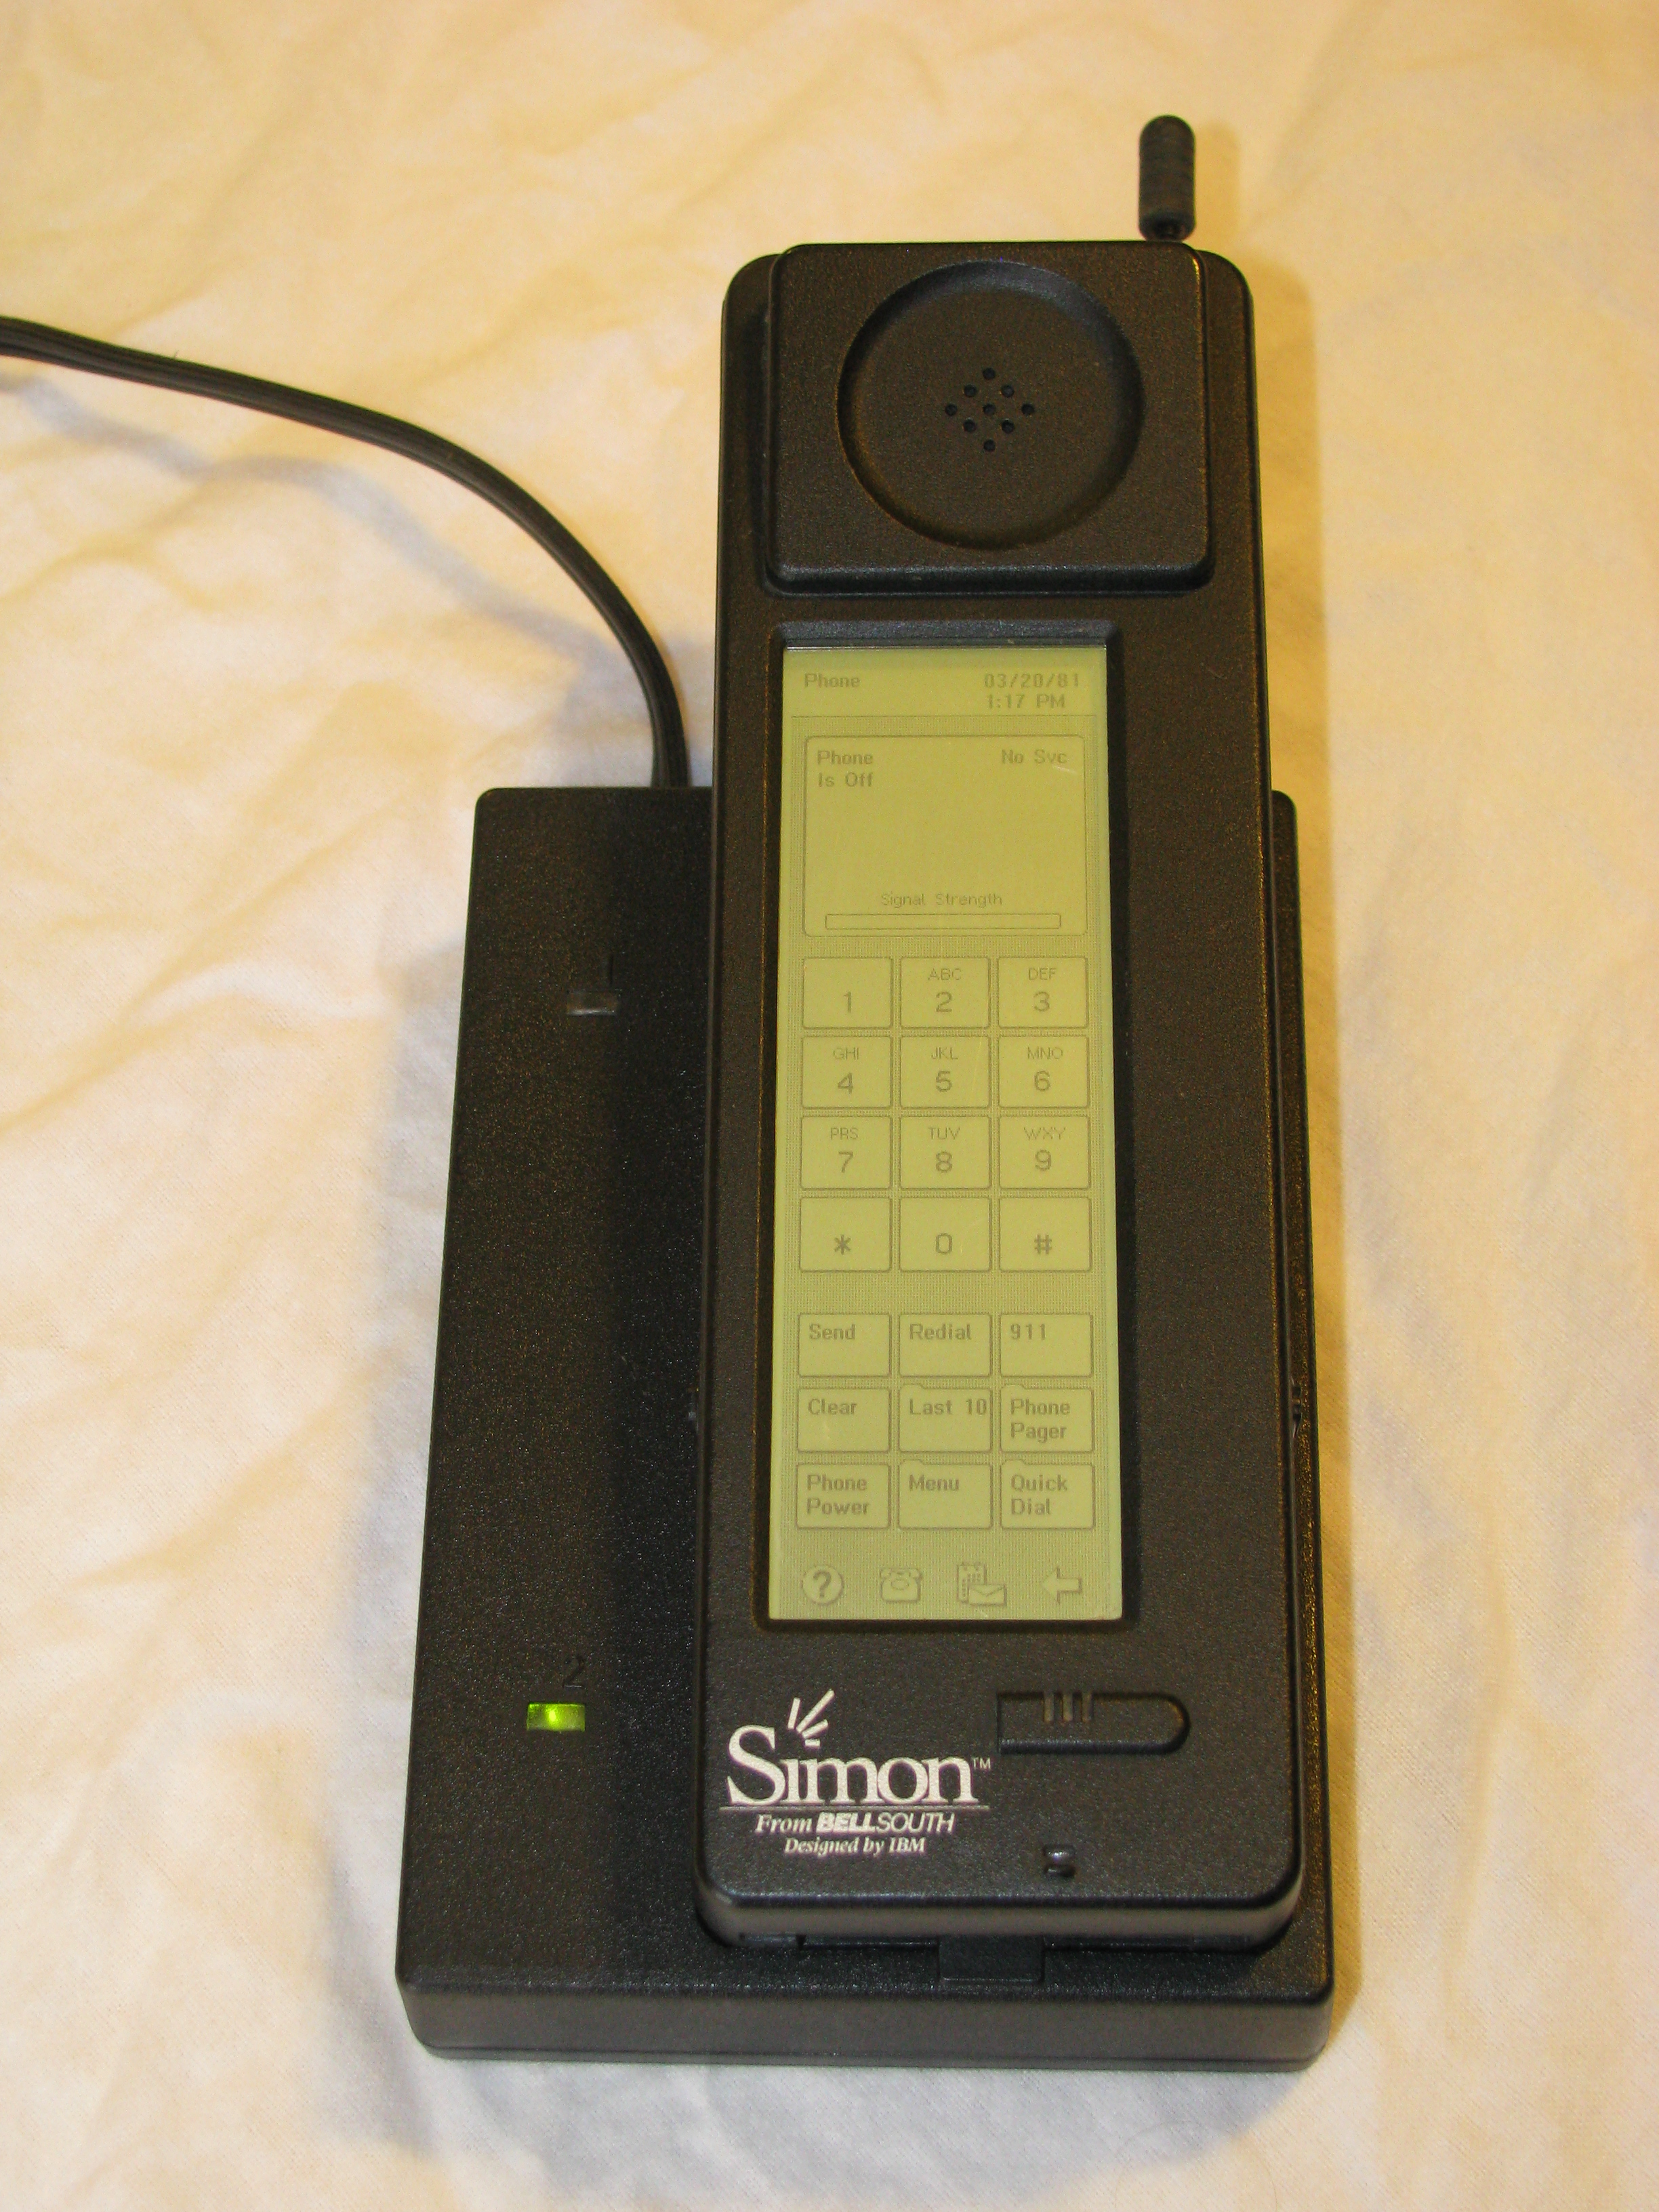
\includegraphics[height=3.7cm]{smart_no1}} \hfill
	\subfloat[Nokia 9210]{\label{picSmart_no2}\includegraphics[height=3.7cm]{smart_no2}} \hfill
	\subfloat[HTC Dream]{\label{picSmart_no3}\includegraphics[height=3.7cm]{smart_no3}} \hfill
	\label{picRS232}
\end{figure}
Pametni telefoni so mobilni telefoni, ki pa ne omogočajo le telefoniranja in pisanja sporočil, temveč ponujajo tudi naprednejše računalniške sposobnosti. Lahko bi rekli da so kot zelo majhni osebni računalniki z malo manj svobode. V večini primerov so pametni telefoni brez tipkovnice in se jih upravlja le na dotik na zaslon. Prvi pametni telefon je bil predstavljen leta 1992 in sicer IBM-ov Simon, ki pa so ga leto pozneje že postavili na trg. Leta 2000 so razvili odprtokodni operacijski sistem Symbian. Na projektu je sodelovalo veliko razvijalcev in sicer {\tt Nokia}, {\tt Sony Ericsson}, {\tt NTT DoCoMo} in {\tt Symbian Ltd.}. S tem se je začela prava doba pametnih telefonov. V dveh letih so na trg prišli še trije operacijski sistemi: {\tt Palm}, {\tt Windows} (Microsoft) in {\tt RIM} (BlackBerry). Operacijska sistema RIM in Windwos sta se zelo hitro razširila po svetu. V zadnjem času sta na trg prišla še dva nova operacijska sistema, ki sta potrebovala za tako majhno napravo zelo zmogljivo strojno opremo. Temu je bila tudi seveda primerna cena. To sta bila {\tt iOS} (Apple) s telefonom iPhone in odprtokodni operacijski sistem {\tt Android} (Google) s telefonom HTC Dream (T-Mobile G1). Čeprav sta bila telefona razmeroma draga je prodaja poskočila, kot je prikazano na sliki~\ref{picsmartProdaja}. Do danes se je cena Android telefonov kar umirila, kar pa ne moremo trditi za iPhone. Obstajajo pa seveda tudi Android telefoni, ki so zelo blizu cene iPhone-a. Cena je odvisna od strojne opreme telefona.~\cite{bibSmartPhoneWiki}

\begin{figure}[h]
	\centering
	\includegraphics[width=5cm]{smartProdaja}
	\caption{Prodaja pametnih telefonov leta 2011~\cite{bibSmartPhoneWiki}}
	\label{picsmartProdaja}
\end{figure}

Za naš problem smo si izbrali telefon z odprtokodnim sistemom Android. Lahko bi si izbrali tudi iPhone ali Windows ampak je Android enostaven za razvoj in še bolj pomembno, odprtokoden. Kot testni telefon smo imeli HTC Desire Z, znan tudi kot T-Mobile G2. Je nadgradnja prvega Android telefona in kar je najpomembnejše pri Gx seriji, ima zunanjo tipkovnico. 

\section{Operacijski sistem Android}
Android je odprtokodni sistem za pametne telefone, ki ga je izdelal {\tt Open Handset Alliance} pod vodstvom {\tt Google}-a leta 2007. Projekt se imenuje AOSP (Android Open Source Project) in se še danes hitro razvija.

Vse skupaj temelji na jedru Linux, najbolj bistven del arhitekture pa je navidezni stroj (ang. virtual machine). Bolj podrobna zgradba sistema je prikazana na sliki~\ref{picAndroid}. Navidezni stroj, imenovan {\tt Dalvik virtual machine}, vsebuje prevajalnik JIT (ang. just-in-time compiler), ki je zadolžen za zaganjanje {\tt Java}nske že prevedene kode. Prevedena koda je zapakirana v datoteke {\tt .apk} in tej datotekam pravimo program, izdelan za sistem Android.

\begin{figure}[h]
	\centering
	\includegraphics[width=0.9\textwidth]{android}
	\caption{Struktura operacijskega sistema Android~\cite{bibAndroidWiki}}
	\label{picAndroid}
\end{figure}
\clearpage

Za izdelavo Android aplikacije potrebujemo znanje programskega jezika {\tt Java}, {\tt Android SDK}, ki je brezplačno na voljo na uradni spletni strani\footnote{Uradna spletna stran je dostopna na {\tt http://developer.android.com/sdk/}~\cite{bibAndroid}}, priporočljivo je tudi branje {\tt SDK dokumentacije}, ki je na voljo na spletu\footnote{SDK dokumentacija je dostopna na {\tt http://developer.android.com/reference/}~\cite{bibAndroid}}. Dokumentacija je napisana razločno, tako da se lahko znajdejo tudi začetniki. S pomočjo Android SDK na koncu nastane .apk.

\subsection{Integrirano razvojno okolje} 
Za vsak večji projekt se ne programira v osnovnem urejevalniku besedil, na primer beležnica (ang. notepad), ampak se za to uporablja integrirano razvojno okolje (ang. integrated development environment - IDE). IDE je programski paket, ki je namenjen programiranju  in obsega urejevalnik besedil, prevajalnik (ang. compiler), povezovalnik (ang. linker), razhroščevalnik (ang. debugger), posnemovalnik (ang. emulator), avtomatsko iskanje možnih ukazov (ang. autocomplete), možnost nalaganja vtičnikov (ang. plug-in) in še veliko lastnosti, ki so nam pri programiranju zelo v pomoč. 

\begin{figure}[h]
	\centering
	\subfloat[NetBeans]{\label{picIde_no1}\includegraphics[height=2.5cm]{ide_no1}} \hfill
	\subfloat[Eclipse]{\label{picIde_no2}\includegraphics[height=2.5cm]{ide_no2}} \hfill
	\subfloat[JDeveloper]{\label{picIde_no3}\includegraphics[height=2.5cm]{ide_no3}} \hfill
	\caption{Različna integrarana razvojna okolja za programski jezik Java}
	\label{picIDE}
\end{figure}

Za Android je priporočljivo razvojno okolje {\tt Eclipse}, ker je zanj narejen vtičnik {\tt ADT Plugin}. 
Eclipse je, kot večina orodij v tem diplomskem delu, odprtokoden, razvija pa ga {\tt Eclipse Foundation}. Napisan je v programskem jeziku Java in se tudi v večini se uporablja za programiranje v Javi. Na voljo je za vse operacijske sisteme, ki so na voljo za osebni računalnik, to so Windows, Linux, Mac OS X in Solaris. Na uradni spletni strani\footnote{Uradna spletna stran je dostopna na {\tt http://www.eclipse.org/}~\cite{bibEclipse}} so različne možnosti paketov programa Eclipse, razlikujejo se le po številu in vrsti vgrajenih vtičnikov. 

Ker potrebujemo le programski jezik Java, je v diplomskem delu u\-po\-rab\-ljen paket Classic. Ta paket vsebuje vse vtiče, ki so potrebni za lažje delo v programskem jeziku Java. Poleg njega potrebujemo že zgoraj napisani ADT Plugin, to je vtič, ki nam na prijazen način omogoči programiranje za Android. Vse kar ta vtič potrebuje je nastavljena pot do Android SDK. Ko ustvarimo nov projekt nam vtič naredi {\tt .xml} datoteko za uporabniški vmesnik, ki je viden na telefonu in {\tt .java} datoteko, kjer se nahaja vsa programska koda. Na novo ustvarjen projekt že vsebuje prevedljiv začetniški program {\tt Hello World}. Uporabnosti v začetnem programu ni, je pa dovolj dober da lahko testiramo prevajanje in zagon programa na telefonu. Namesto telefona nam Android SDK omogoča tudi posnemovalnik telefona, ampak je v primerjavi s telefonom zelo počasen. Posnemovalnik je lahko katerekoli ločljivosti (ang. resolution) in lahko testiramo tudi za telefone, katerih si ne lastimo. Kljub temu, da je posnemovalnik dobra alternativa, je testiranje s pravim telefonom zelo priporočljivo. 

\section{Aplikacija za vodenje mobilne platforme}
Program za to diplomsko delo smo poimenovali Roomba. V tem programu želimo doseči povezavo za zgoraj opisani usmerjevalnik Linksys WRT54GL preko ssh povezave. Za ssh smo se odločili zato, ker jo usmerjevalnik že vsebuje in ker je dovolj varna in stabilna povezava. V pomoč nam je prišla že narejena knjižnjica {\tt JSch}\footnote{Knjižnica je dostopna na {\tt http://www.jcraft.com/jsch/}~\cite{bibJcraft}}. S pomočjo JSch smo vzpostavili ssh povezavo, in ob potrebi poslali ukaz, ki se nato izvede v ukazni lupini (ang. shell) usmerjevalnika. Za vzpostavitev povezave potrebujemo IP naslov, uporabniško ime in geslo usmerjevalnika, ki jih vnesemo preko uporabniškega vmesnika nastavitev, kot je prikazano na sliki \ref{picAndroidPref}. Uporabniško ime ima OpenWRT privzeto nastavljen kot {\tt root} in ima pravico do celotnega sistema OpenWRT, geslo si pa nastavimo sami ob prvem zagonu usmerjevalnika. V našem projektu izmed vseh pravic koristimo le zagon programa Roombacmd. 

\begin{figure}[h]
	\centering
	\includegraphics[width=0.75\textwidth]{androidPref}
	\caption{Možne nastavitve v programu Roomba}
	\label{picAndroidPref}
\end{figure}

Poleg ssh povezave potrebujemo tudi tok podatkov (ang. data stream) za podatke iz IP kamere. Tok podatkov IP kamere se prenaša v formatu Motion JPEG. Ker android SDK ne vsebuje primerne komponente za predvajanje tega formata, ampak dovoljuje le prikaz posamezne slike, potrebujemo novo grafično komponento. Skupina ljudi se je tega problema že lotila in naredila odprtokodni projekt android-camera-axis\footnote{Projekt je dostopen na {\tt http://code.google.com/p/android-camera-axis/}}. Njihovo komponento smo optimizirali zahtevam, ki jih potrebujemo za prikaz slike, in ji s tem odstranili veliko nam neuporabnih možnih nastavitev. Glavno nastavitev, to je nastavitev IP naslova kamere, smo pustili in jo tudi nastavili v istem trenutku kot, vzpostavimo ssh povezavo. Tok podatkov iz kamere se je nato prikazal čez celoten zaslon telefona (ang. full screen). S tem so bile vse zunanje povezave vzpostavljene in potrebujemo le še parametre za vodenje naše mobilne platforme. 

Parameter za smer smo upravljali tako kot večina dirkaških igric na telefonu. Da je vse skupaj bolj realistično uporabljamo telefon kot volan v avtomobilu. To nam omogočajo senzorji v telefonu, ki zaznajo za koliko je telefon nagnjen glede na zemeljsko površino (ang. accelerometer) za vse tri koordinate ampak ker potrebujemo le smer levo in desno potrebujemo le y koordinato. Razpon vsake koordinate sega od -10 do 10 na več decimalnih mest natančno, naša mobilna platforma pa ima razpon smeri celoštevilski od -2000 do 2000. 

Drugi parameter, to je parameter za hitrost, je dobljen s pomočjo že narejene grafične komponente SeekBar. SeekBar je komponenta narejena na osnovi komponente ProgressBar, ki se najpogosteje se uporablja za grafični prikaz napredka kakšne dolge operacije. Glavna pridobitev SeekBar je drsnik, s katerim uporabnik nastavi pozicijo, to je napredek. V našem projektu ni uporabljen za prikaz napredka, temveč za nastavitev hitrosti. Višje kot je nastavljen drsnik, z večjo hitrostjo drvi naša mobilna platforma. Razpon napredka smo nastavili glede na razpon mobilne platforme, to je od 1 do 500. Dodali smo še dodatnih 11 stopenj razpona in sicer 0 za ustavitev in od -1 do -10 za negativno hitrost, kar pomeni da se bo mobilna platforma premikala vzvratno. 

Na sliki~\ref{picAndroidApp} so prikazane vse zgoraj opisane komponente. Čez cel zaslon opazimo sliko iz IP kamere, ki se prilagaja ne glede na resolucijo telefona. Na desnem robu je napisana številka, ki pomeni, da bo mobilna platforma zavila za 1521mm v desno, zato je tudi prikazana na desnem robu. 

\begin{figure}[h]
	\centering
	\includegraphics[width=0.65\textwidth]{androidApp}
	\caption{Program Roomba v teku}
	\label{picAndroidApp}
\end{figure}

Če bi telefon nagnili malo bolj levo bi se napis prestavil na levi rob in mobilna platforma bi začela zavijati levo. Večja kot je številka, manjši zavoj bo izveden. Spodaj desno pa opazimo SeekBar, namenjen hitrosti. Trenutno je nastavljen na hitrost 0, če premaknemo drsnik, to je bela kroglica, malo nazaj se mobilna platforma počasi premika vzvratno dokler drsnika spustimo, nato se zopet ustavi. To je le varnostni ukrep, ker vzvratno premikanje ni naravno za sesalec Roomba. Ko pa želimo mobilno platformo premikati naprej, nam drsnika ni treba ves čas držati, ga le nastavimo na želeno hitrost in uživamo v vožnji.

\subsubsection{Testiranje programa}
Za testiranje programa Roomba je uporabljen telefon HTC Desire Z.

\begin{figure}[h]
	\centering
	\includegraphics[width=0.5\textwidth]{DZ}
	\label{picDZ}
\end{figure}

{\tt HTC Desire Z} je pametni telefon, ki ga je izdelal HTC Corporation. Izšel je novembra 2010 in je mnogo uporabnikov starega HTC Dream prepričal v zamenjavo za le-tega. Kot vsi HTC-jevi android telefoni je tudi HTC Desire Z opremljen s {\tt HTC Sense}, ki je namizno okolje operacijskega sistema (angl. graphical user interface). Namizno okolje HTC Sense in AOSP je tako različno, da bi na prvi pogled težko prepoznal isti operacijski sistem. Zaradi zmogljive strojne opreme je bi dovolj močan za prejemanje slike iz kamere, kar pri telefonu zelo zahtevno.

\chapter{Delovanje sistema}
Preko celotnega dela se je sistem močno razširil, kar je tudi mogoče opaziti na sliki~\ref{diaSistem}. 

\begin{figure}[h]
	\centering
	\includegraphics[width=0.75\textwidth]{sistem}
	\caption{Celoten sistem}
	\label{diaSistem}
\end{figure}

Usmerjevalniku je dodan nov konektor za zaporedna vrata, ki je preko pretvornika, iz RS232 na ROI, vezan na ROI vmesnik, ki je že v osnovi na sesalcu Roomba. S tem je dosežena povezava, ter komunikacija med mobilno platformo in zunanjim svetom. Na usmerjevalnik je priključena IP kamera in je s tem posledično tudi povezana v zunanji svet. Na neki drugi lokaciji v zunanjem svetu imamo pameten telefon, namenjen vodenju prej opisane kombinacije naprav.

Ves sistem delovanja se prične pri povezavi med usmerjevalnikom in telefonom z brezžičnim omrežjem. Uporabljena je varna povezava ssh in, ko je le ta vzpostavljena, ima usmerjevalnik nalogo pošiljati različne nize bitov skozi zaporedna vrata. Zaporedna vrata so s kablom povezana na zaporedna vrata sesalca Roomba. Ker je to žična povezava, je posledično usmerjevalnik pritrjen na sesalec. Na usmerjevalnik je preko mrežnega kabla povezana tudi IP kamera, ki je prav tako pritrjena na sesalec. Ker pa usmerjevalnik in kamera potrebujeta tudi zunanje napajanje je dodana še 7Ah baterija. Baterija je uporabljena, da nadomesti nekaj metrov dolg kabel, ki je bil na začetku uporabljen za pridobivanje zunanjega napajanja. S tem smo dosegli večjo mobilnost, razlika pa je razvidna na sliki~\ref{picKoncano}.

\begin{figure}[h]
	\centering
	\subfloat{\label{picKoncano_no1}\includegraphics[width=0.45\textwidth]{koncano_no1}} \hfill
	\subfloat{\label{picKoncano_no2}\includegraphics[width=0.45\textwidth]{koncano_no2}} \hfill
	\caption{Razlika med končanim sistemom z zunanjo baterijo (desno) in brez (levo)}
	\label{picKoncano}
\end{figure}

\chapter{Sklepne ugotovitve}
Cilj, ki smo si ga zadali na začetku in je prikazan na sliki~\ref{diaShema} je torej zgrajen. Celoten sistem je opremljen s štirimi skoraj vsakdanjimi komponentami, ki so uporabljene na drugačen način kot v vsakdanjem življenju z izjemo IP kamere, katera nima druge funkcije kot je oddajanje zaporedja slik.

Začnimo z sesalcem Roomba, ki je avtomatski sesalec. Namesto običajnega avtomatskega sesanja je uporabljen kot vodljivo prevozno sredstvo. Njegova naloga je voziti z različno hitrostjo v vse smeri, omejen je le na ravno površino, kjer ga lahko zunanje upravljamo. 

Usmerjevalnik Linksys WRT54GL se v vsakdanjem življenju uporablja kot brezžični usmerjevalnik, na katerega se lahko več osebnih računalnikov poveže žično ali brezžično. Tukaj je ravno obratno, saj se sam obnaša kot računalnik in se poveže na drug usmerjevalnik, s čimer je zagotovljena povezava z zunanjim svetom.

Telefon se uporablja za telefoniranje in podobno, v tem primeru pa je uporabljen podobno kot igralna konzola za igrice za upravljanje mobilne platforme preko uporabniškega vmesnika. 

Obstaja še veliko dobrih lastnosti, ki jih omogočajo komponente našega sistema. Že samo z uporabo senzorjev sesalca Roomba lahko dosežemo, da nas, na primer opozarja na morebitne nevarnosti na poti, ki smo jih spregledali na kameri. Možno je tudi dodajanje novih senzorjev, na primer senzor za dež, toploto, ... kot smo mi dodali kamero. Za nadaljnje delo je odprto mnogo poti in vsaka pot ima svoj smisel. 

\begin{thebibliography}{99}
\bibitem{bibHackRoomba} Tod E. Kurt, ``Hacking Roomba'', John Wiley \& Sons,  Indianopolis, Indiana,  2007
\bibitem{bibKamera} Uradna spletna stran kamere AXIS 215 PTZ
Dostopno na: http://www.axis.com/products/cam\_215/ (zadnji obisk 10.09.2011)
\bibitem{bibWikiRoomba}Roomba, Wikipedija \\
Dostopno na: http://en.wikipedia.org/wiki/Roomba (zadnji obisk 10.09.2011)
\bibitem{bibOpenWRT} Uradna spletna stran OpenWRT \\
Dostopno na: http://wiki.openwrt.org/ (zadnji obisk 10.09.2011)
\bibitem{bibSmartPhoneWiki} Smartphone, Wikipedija \\
Dostopno na: http://en.wikipedia.org/wiki/Smartphone/ (zadnji obisk 10.09.2011)
\bibitem{bibAndroidWiki} Android, Wikipedija \\
Dostopno na: http://en.wikipedia.org/wiki/Android\_(operating\_system)/ (zadnji obisk 10.09.2011)
\bibitem{bibAndroid} Uradna spletna stran za razvijalce Android \\
Dostopno na: http://developer.android.com/ (zadnji obisk 10.09.2011)
\bibitem{bibJbproject} Uradna spletna stran jbproject \\
Dostopno na: http://www.jbprojects.net/articles/wrt54gl\_mods/ (zadnji obisk 10.09.2011)
\bibitem{bibRoombaROI} Uradna spletna stran HackingRoomba \\
Dostopno na: http://hackingroomba.com/projects/build-a-roomba-serial-tether/ (zadnji obisk 10.09.2011)
\bibitem{bibRoombacmd} Uradna spletna stran Roombamd \\
Dostopno na: http://hackingroomba.com/?s=roombacmd (zadnji obisk 10.09.2011)
\bibitem{bibEclipse} Uradna spletna stran Eclipse \\
Dostopno na: http://www.eclipse.org/ (zadnji obisk 10.09.2011)
\bibitem{bibJcraft} Uradna spletna stran Jcraft \\
Dostopno na: http://www.jcraft.com/ (zadnji obisk 10.09.2011)
\end{thebibliography}
\end{document}